%\documentclass[a4paper,12pt]{article}
\documentclass[english,authoryear]{elsarticle}
\usepackage{apalike}
\usepackage{graphicx}
\usepackage[T2A]{fontenc}
\usepackage[utf8]{inputenc}
\usepackage{csquotes}
\usepackage[russian,english]{babel}
%\usepackage{apacite}
\usepackage{amsmath,amsfonts,amssymb,amsthm,mathtools} % AMS
\usepackage{listings}
%\usepackage{gensymb}
\usepackage{xcolor}
\usepackage[version=3]{mhchem}
\usepackage{makecell}
\usepackage{gensymb}
%\usepackage[colorlinks,allcolors=cyan!70!black]{hyperref}
\renewcommand\theadalign{bc}
\renewcommand\theadfont{\bfseries}
\renewcommand\theadgape{\Gape[4pt]}
\renewcommand\cellgape{\Gape[4pt]}

\title{Cytoskeletal and motility changes in human mesenchymal stem cells associated with nuclear-cytoplasmic RhoА redistribution during replicative aging}
\begin{document}
\date{today}

\author[rvt]{Danila Bobkov\corref{cor1}}
\ead{bobkov@incras.ru}
\author[add]{Anastasia Polyanskaya}
\author[rvt]{Anastasia Musorina}
\author[rvt]{Ekaterina Lomert}
\author[rvt]{Sergey Shabelnikov}
\author[rvt]{Galina Poljanskaya}
\cortext[cor1]{Corresponding author}
%\author{Danila Bobkov, Anastasia Polyanskaya, Anastasia Musorina, Ekaterina Lomert, Sergey Shabelnikov, Galina Polyanskaya}
%\affil[1,2,3]{Institute of Cytology of the Russian Academy of Science, 194064 Tikhoretsky ave. 4, St-Petersburg, Russia}
\address[rvt]{Institute of Cytology of the Russian Academy of Science, 194064 Tikhoretsky ave. 4, St-Petersburg, Russia }
\address[add]{Centre for Study of Things}


\begin{abstract}
Here we provide evidence.
The analysis of data from measurements is analyzed.
\end{abstract}

\begin{keyword}
mesenchymal stem cells\sep senescense\sep actin\sep myosin-9\sep RhoA\sep cell motility.
\end{keyword}

\maketitle
\section{Introduction}

At present, the urgent task of cell biology is the isolation and comparative characterization of human mesenchymal stem cells (MSCs) isolated from various sources.
The importance of such studies stems from the features of the interaction of MSCs isolated from different tissues, with their characteristic microenvironment.
The origin or source of the MSC can determine their functional characteristics.
Comparative analysis of the characteristics that are decisive in maintaining the status of MSCs, as well as a number of other characteristics responsible for the most important cellular processes, contributes to the deepening of basic knowledge of human MSCs, which is important both for understanding the mechanisms of biological processes in the cell and for expanding opportunities for using MSCs in regenerative medicine.
Due to the importance of MSC for the functioning of the body, the mechanisms of MSC interaction with damaged tissues and organs are widely studied.
It has been shown that one of the most important mechanisms of action of various MSCs on damaged tissues is their ability to migrate to these sites and exert a trophic action due to the secretion of bioactive factors that alter the microenvironment of damaged cells and, thereby, improving tissue repair.
At present, the mechanisms of tissue repair using MSCs related to the production of cytokines and paracrine factors are widely discussed in the literature (\cite{phinney2007concise}; \cite{m2011mesenchymal}; \cite{guiducci2011bone}; \cite{gruenloh2011characterization}; \cite{huang2013effects}; \cite{luo2013mesenchymal}; \cite{ando2014stem}; \cite{hendijani2015human}; \cite{hendijani2015effect}; \cite{danieli2016testing}; \cite{julianto2016topical}; \cite{teixeira2017impact}; \cite{vulcano2016wharton}; \cite{zachar2016activation}).


Non-immortalized cell lines undergo a process of replicative aging.
Replicative aging is a complex process that can begin at the early passages and gradually increase in the process of long-term cultivation.
It is characterized by a significant decrease or cessation of proliferation, shortening of telomeres, morphological changes, increased $\beta$-galactosidase activity, increased expression of the tumor suppressor genes, decreased DNA repair and antioxidant activity of aging cells, due to reduced expression of the corresponding genes, decreased differentiation potential, a number of epigenetic changes (\cite{wagner2008replicative}; \cite{kuilman2010essence}; \cite{redaelli2012cytogenomic}; \cite{estrada2013human}; \cite{savickiene2016senescence}; \cite{danisovic2017effect}; \cite{koltsova2018dynamics}; \cite{alessio2018mesenchymal}; \cite{krylova2018isolation}; \cite{niedernhofer2018nuclear}; \cite{truong2018characterization}; \cite{yu2018replicative}).

It is important to emphasize that aging of MSCs may be associated not only with replicative aging, which can be traced during prolonged passaging of MSCs in vitro, but also with factors external to MSCs.
Aging mechanisms affect both MSCs and microenvironment.
In this regard, it is the interaction of MSCs and the microenvironment that ensures the age characteristics of MSCs (\cite{sethe2006aging}).
One of the essential signs of replicative aging is a decrease in cell motility or cell migration (\cite{geissler2012functional}; \cite{bertolo2015vitro}; \cite{turinetto2016senescence}; \cite{zhang2018overexpression}).
Violation of migration processes contributes to the deterioration of tissue repair.
Therefore, to use MSCs in regenerative medicine, it is necessary to know the nature of the process of replicative aging in a particular line.
It is important to understand which passages are most suitable for using aging cell cultures for biomedical work.


Cell migration occurs through close contact with the extracellular matrix, on which cells are spread, and depends on the organization of the actin cytoskeleton.
In this regard, it is essential to study the role of aging in the organization of the cytoskeleton.
There are a number of works describing molecular mechanisms and functional changes during the reorganization of the cytoskeleton during replicative aging in different human and animal cell types (\cite{larsen2003phosphatases}; \cite{le2008regulation}; \cite{wang2009protein}; \cite{geissler2012functional}; \cite{ozcan2016unbiased}; \cite{turinetto2016senescence}; \cite{moujaber2019cellular}).
Currently, studies on the effect of replicative aging on cytoskeleton reorganization are at the stage of accumulation of experimental results.
It is of considerable interest to analyze the effect of replicative aging on cell motility and the reorganization of the actin cytoskeleton in the human MSC line, which has not been used in detail in such studies.


Currently, much attention is paid to the selection of MSCs from extra-embryonic organs, which are formed in the first weeks of pregnancy, because obtaining MSCs from these organs is not associated with a number of restrictions in obtaining MSCs from other tissues: an invasive method of production and ethical problems (\cite{bongso2013therapeutic}).
Previously, we obtained a non-immortalized human cell line from the Varton's jelly umbilical cord, called MSCWJ-1.
The analysis of the main characteristics confirming the status of MSCs for it, according to the requirements of the International Society for Cellular Therapy (\cite{dominici2006minimal}; \cite{sensebe2010mesenchymal}; \cite{krylova2017derivation}).


Thus, the objective of this study is analysis of replicative aging in the process of long-term cultivation of the MSCWJ-1 in terms of the actin cytoskeleton structure and the behavior of moving cells.


The hypothesis of this study was that motility changes associated with human MSC senescence are actin-cytoskeleton and RhoA-dependent.
Little is known about how the structural aspects of these cells are modified as a result of replicative aging.
Using fluorescence and confocal microscopy-based quantitative image cytometry techniques, we investigated changes in distribution of F-actin and actin-binding proteins myosin-9 and $\alpha$-actinin-4 as well as small GTPase RhoA in conjunction with the registration of parameters characterizing cell motility.
In order to characterize the change in the composition of cytoplasmic protein complexes containing myosin-9 and beta-actin, we used liquid chromatography.



\section{MATERIALS AND METHODS}

\subsection{Cell cultures: MSCWJ-1}

A line of human mesenchymal stem cells obtained from Varton's jelly of the umbilical cord of the person (MSCWJ-1) was used in the work.
The characterized cell line was obtained from "Collection of vertebrate cell cultures" of the Institute of Cytology of the Russian Academy of Sciences (St. Petersburg, Russia).
MSCWJ-1 cells were cultured in growth medium containing 90\% DMEM/F12 medium (Biolot, Russia) and 10\% fetal bovine serum (FBS) (Hyclone, United States).
Cells were cultured in 5\% $CO_2$, $37\degree C$ and 90\% humidity conditions.
Microbiological analysis confirmed the absence of bacterial, fungal and mycoplasmal contamination in the resulting line.
The cultivation method was monolayer reseeding, the reseeding procedure consists in removing the cells with 0.25\% trypsin, the multiplicity of sieving is 1:3, optimum density of cell suspension was 5.0 x $10^{6}$ cells/ml.

\subsection{Replicative cell aging}

The efficacy of the $\beta$-galactosidase enzyme was evaluated by the $\beta$-galactosidase enzyme activity.
MSCWJ-1 cells were grown in 3.5 cm Petri dishes until subconfluent formation.
Then the medium was removed and the cells were stained using a reagent kit (Senescence $\beta$-galactosidase staining kit; Cell Signaling, USA), according to the instructions.
In cells entering the phase of replicative aging, the cytoplasm has a bright blue color.
The analysis was performed using an inverted microscope equipped with 60x objective (Nicon, Japan) on the 6th, 15th, 20th and 28th passages.
The percentage of stained cells in percent was determined by counting at least 1000 cells in different fields of view at one time point.
The results were processed statistically using Wilson method to compute 95\% confidence intervals for binomial proportions.

\subsection{Immunofluorescence}

Coverslips with adherent cells were fixed in a 3\% solution of paraformaldehyde for 10 min at room temperature and permeabilized in a solution of 0.1\% TritonX-100 for 10 min at room temperature, then the coverslips with cells was poured with 1\% BSA solution for 20 min.
Rabbit polyclonal antibodies produced against the N-terminal peptide of the heavy chain of nonmuscle myosin IIA, rabbit polyclonal antibodies produced against the $\alpha$-actinin-4 and mouse monoclonal antibodies produced against the RhoA were used as the first antibodies.
Goat antibodies to the Alexa fluor 488 rabbit antigens (Invitrogen, USA) were used as second antibodies.
To visualize the actin cytoskeleton, cells were stained with rhodamine phalloidin for 20 min at room temperature and stained with DAPI with final concentration 1.5 $\mu$g/mL.
Preparations were made on ProLong Gold antifade reagent containing.
Cells were analyzed on a confocal microscope Leica SP8 (Germany).


\subsection{Colocalization analysis}

Colocalization coefficients were calculated using ImageJ version 1.52i using the Coloc 2 plugin (\cite{rueden2017imagej2}).
Raw 1024 x 1024 px images was in 72 dpi resolution.
For colocalization analysis images were opened in ImageJ, RGB channels were converted to 32 bit grayscale.
Cells were selected manually on merged image and ROI passed to Coloc 2 plugin.
The Pearson, Spearman, Manders and Kendall colocalization coefficients were calculated and passed as CSV files to R environment.
However, Pearsons correlation coeff can be pretty noisy (\cite{adler2008replicate}; \cite{bergholm2010analysis}).
For further analysis, the values of the $\tau$-Kendall rank correlation coefficient (bTau) and Pearson product-moment correlation coefficient (Rval) were used.
The values of the correlation coefficient bTau were interpreted in accordance with the Cheddock scale (see table \ref{cheddock}).

\begin{table}[h]
  \caption{Cheddock scale}
  \label{cheddock}
\centering
\begin{tabular}{l|c|}
  bTau Value & Colocalization \\
 \hline
 $ <0.1 $ & no link \\
 0.1-0.3 & weak \\
 0.3-0.5 & moderate \\
 0.5-0.7 & noticeable \\
 0.7-0.9 & high \\
 0.9-0.99 & very high
\end{tabular}
\end{table}



\subsection{Quantitative image cytometry and cell movement analisys}

Comparative analysis of cell movement characteristics relative to replicative aging was performed using time-lapse movies.
For recording the movement of individual cells we used high-content Quantitative Image Cytometer CQ1 (Yokogawa) with Nipkow spinning disk confocal technology (\cite{sakashita2015cq1}).
Cells were plated on 6-well dishes and stained with Hoechst 33342 (Invitrogen, USA).
Images were acquired during 24 h session with 405-nm laser and bright field illumination using 40x 0.95-NA dry objective lens.
All images had a 2560 x 2160 pixel resolution, with a pixel size equivalent to 0.2 $\mu$m in x and y.
A set of x-y coordinates were obtained from images in ImageJ software with Manual tracking plugin.
Each cell was manually marked in the middle of the nucleus in each time point.
Only cells satisfying the following conditions were noted: the cell must be in the field of view in all frames, the cell does not divide.
Dividing cells were not counted.
Trajectories were obtained from from a set of x-y coordinates.
The resulting tracks were combined into a data frame and analyzed in the R environment using trajr package (\cite{mclean2018trajr}), which is a sutable toolkit for the numerical characterisation and analysis of the trajectories of moving cells.
Trajectory coordinates were read from a CSV data file, and then passed in to the trajectory analysis functions.
Trajectorys was resampled to 15 min fixed step lenght by rediscretization function using the algorithm described by Bovet & Benhamou (\cite{bovet1988spatial}).
As a result of the analysis of the trajectories, we obtained the following parameters: total length of the trajectory, straight-line distance from the start to the end of the trajectory, mean and maximum speeds, straightness and sinuosity indexes.
To measure the straightness, or conversely, tortuosity, of trajectories, we used two indexes.
The simplest is straightness index and computed as D/L, where D is the distance from the start to the end of the trajectory, and L is the length of the trajectory.
This straightness index is a number ranging from 0 to 1, where 1 indicates a straight line.
The straightness index is considered to be a reliable measure of the efficiency of a directed walk, but inapplicable to random trajectories (\cite{benhamou2006detecting}).
The sinuosity index defined by Benhamou (\cite{benhamou2004reliably}) may be an appropriate measure of the tortuosity of a random search path.
Sinuosity is a function of the mean cosine of turning angles, and is a corrected form of the original sinuosity index defined by Bovet and Benhamou (\cite{bovet1988spatial}).

\subsection{FPLC gel filtration}

We obtained cell extracts by lysis from a monolayer cell culture grown on 14 Petri dishes 9 cm in diameter.
In order to prevent the destruction of multimolecular protein complexes, in the first stage the medium in the plates was replaced with medium containing 10 $\mu$M formaldehyde, incubated for 10 minutes at 37 $\degree$ C, then a solution of glycine at a concentration of 1.875 g per 200 ml was added to each cup PBS, incubated for 5-7 min at 37 $\degree$  C. Subsequently, we washed the cups after glycine with a solution of PBS and poured 20 $\mu$l of protease inhibitor and 1 ml of lysis buffer was left for 1 min on ice.
Next, the method of sequential selection of cell extract was collected in the ependorf 1 ml of the sample. The final stage of lizing was centrifugation for 10 min at 24000 relative centrifugal force (RCF) and freezing of the samples at -80 $\degree$  C.


For gel-chromatographic separation of cell lysates, an FPLC system (Pharmacia) was used.
Signal detection was performed using Millichrome A-02 detection unit.
Elution was performed with elution buffer (150 mM NaCl, 50 mM Tris, pH 7.5, 0.02\% NaN3).
The column was calibrated with the set of proteins shown in table
\ref{calibration}.


The protein extract was filtered and applied to the column in a volume of 500 $\mu$l.
Fractions were collected on ice 1 ml each 2 min starting from time point determined by calibration set separation.
For protein sedimentation, 100 $\mu$l of 0.15\% DOX sodium deoxycholate was added to the collected fractions and mixed vigorously, incubated for 10 minutes in a refrigerator, then 100 $\mu$l of 50\% TCA was added, mixed, incubated for 15 minutes in a freezer, and precipitated by centrifuging the protein for 30 minutes at 20000 G at +4$\degree$ C.
The supernatant was removed, and cold 100\% acetone was added to the precipitate, mixed vigorously and incubated for 12 hours at -20$\degree$ C.
A repeated washing with acetone was done, and then the protein was precipitated by centrifugation for 15 min at 20000 G at +4$\degree$ C, the supernatant was collected, the precipitate was dried, and 2-fold sample buffer was added to the precipitate (125 mM Tris-HCl, pH 6.8, 4\% SDS, 10\% glycerol, 0.006\% bromo-phenol blue, 1.8\% $\beta$-mercaptoethanol).
Samples were heated for 10 minutes at 98$\degree$ C, probes were stored at -20$\degree$ C before electrophoretic separation.

\subsection{Electrophoresis and western blot}

Proteins were separated by electrophoresis in a 12.5\%  polyacrylamide gel under denaturing conditions in the presence of SDS (\cite{laemmli1970cleavage}).
After electrophoresis, the gel was stained with Coomassie brilliant blue or carried out by Western blotting (\cite{towbin1979electrophoretic}).
Protein transfer from the gel to the Immobilon-P membrane (Millipore, United States) was carried out in Tris-glycine buffer pH 8.3, containing 10\% ethanol and 0.1\% SDS.
Western blotting was performed according to the ECL protocol (Amersham, USA).
After transferring, the membrane was washed for 20 minutes with PBS containing 0.1\% tween-20 and blocked non-specific binding sites with 5\% non-fat dry milk diluted in PBS for 1 hour.
The membrane was incubated with the first antibodies for 1 hour at room temperature three times. washed in PBS, stained with second antibodies for 1 h at room temperature.
Rabbit polyclonal antibodies produced against the N-terminal peptide of myosin-9, mouse monoclonal antibodies produced against the beta-actin were used as the first antibodies.
Rabbit antibodies to mouse antigens and goat antibodies to rabbit antigens conjugated with horseradish peroxidase (Sigma, USA) were used as second antibodies.
To enhance the signal in western blotting, SuperSignal substrate (Thermo Scientific, USA) was used.
Chemiluminescent radiation was recorded using a ChemiDoc system (Bio-Rad, USA).


\subsection{Description of statistical analysis methods}

The study materials were subjected to statistical processing using the methods of parametric and non-parametric analysis.
The accumulation, correction, systematization of the initial information and visualization of the obtained results were carried out in Microsoft Office Excel 2016 spreadsheets.
Statistical analysis was done using the free software computing environment R v. 3.5.3 (\cite{team2014r}).
The data obtained from measurements of the colocalization coefficient were combined into variational series, in which the arithmetic mean values (M) and standard deviations (SD) were calculated.
Those observations that deviate from the 1st or 3rd quartile by more than one and a half interquartile range were considered outliers and deleted.
Quantitative indicators were evaluated for compliance with the normal distribution, for this purpose, the Shapiro – Wilk criterion  was used with $8 < n < 15$ (\cite{shapiro1965analysis}; \cite{shapiro1972approximate}) as well as indicators of asymmetry and kurtosis.
When comparing several samples of quantitative data with a distribution other than normal, Kruskal-Wallis criterion was used, which is a non-parametric alternative to single-factor analysis of variance (\cite{kruskal1952use}).
The Kruskal-Wallis criterion was calculated after ranking all the elements of the analyzed sets.
In the event that the calculated value of the Kruskal-Wallis criterion exceeded the critical one, the differences in the indicators were considered statistically significant.
Otherwise, the null hypothesis was recognized true.
We also used the Wilcoxon W-test to check the differences between the two paired samples compared (\cite{wilcoxon1992individual}).
For each group of measurements, the magnitude of the change in the colocalization coefficient was calculated.
If the calculated value of W was less than or equal to the critical value, it was concluded that the differences of the compared samples were statistically significant.

\subsubsection{Multiple Testing Correction}

In the course of all-pairs comparisons Mann-Whitney rank test, Bonferroni method, Scheffe’s test and post hoc pairwise test for multiple comparisons of mean rank sums (Dunn’s test) were used to adjust the P-values. The results were visualized using the free Python computing software environment and the scikit-posthocs package (\cite{Terpilowski2019}).


\section{RESULTS}

\subsection{$\beta$-Galactosidase activity}


The degree of replicative aging during long-term cultivation of MSCWJ-1 was assessed by the activity of $\beta$-galactosidase in cell populations.
The results are presented in the table \ref{tab} and on the figure \ref{m9-actin-bgal} (E).
The proportion of stained cells naturally increases with aging, which confirms the status of this cell line as aging non-transformed cells.
For definiteness, we assume that the cell lines are old, in which more than 40 percent of the cells in the population stain for beta-galactosidase.


\begin{table}[hb]
  \caption{$\beta$-galactosidase enzyme activity in MSCWJ-1 cells with limits of the 95\% confidence interval}
  \label{tab}
\centering
\begin{tabular}{c|c|c}
 Passage Number & Cells stained for $\beta$-gal,\% & Cell count  \\
 \hline
 9 & 6.02 $\pm$ 0.72 & 3724 \\
 15 & 20.55 $\pm$ 1.57 & 2404 \\
 20 & 26.28 $\pm$ 2.46 & 1149  \\
 28 & 43.97 $\pm$ 2.72 & 1260

\end{tabular}
\end{table}

\subsection{Immunofluorescent cell analysis}

Morphological analysis of the cell line during long-term cultivation showed homogeneity of cell populations with medium-sized elongated fibroblast-like cells at the 9th and 28th passages.
In the process of cultivation, there is a change in the morphology of the cells, expressed in an increase in the size and degree of cell spreading.

In order to assess the changes in the structure of the contractile apparatus that can occur during replicative aging, we investigated the structures of the actin cytoskeleton using rhodamine-phalloidin staining.
Since myosin is a key protein for cell migration.

Fig. \ref{m9-actin-bgal} shows cells stained with antibodies against myosin-9, actin cytoskeleton visualized with rhodamine phalloidin.
In all spread cells, staining for myosin-9 reveals a characteristic striated pattern.

Myosin-9 is distributed along stress-fibrils, striation is often observed along stress-fibrils.


\begin{figure}[hbt!]
  \label{m9-actin-bgal}
\centering
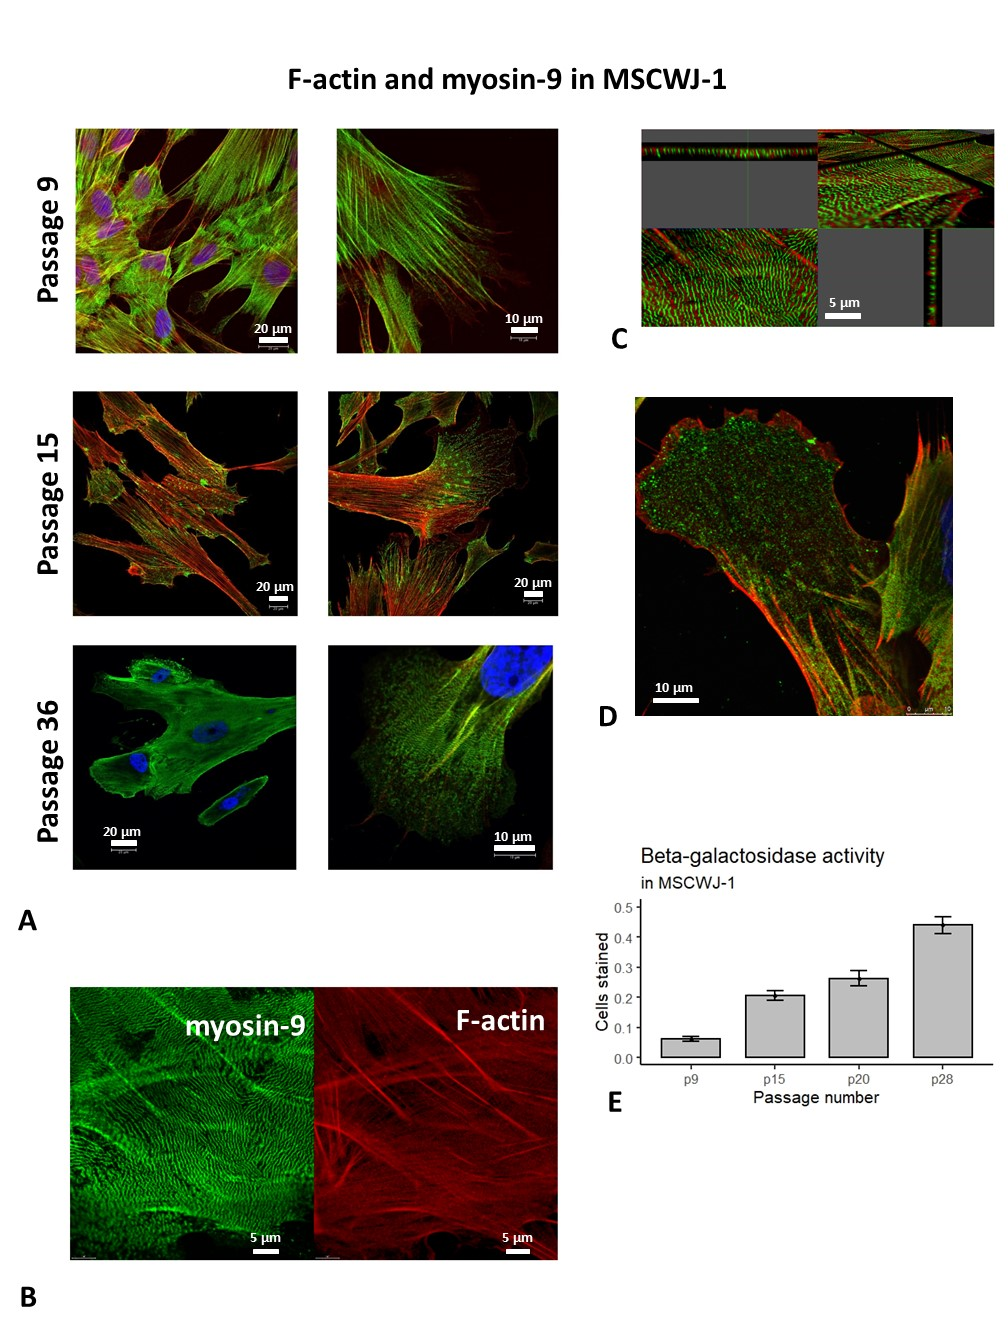
\includegraphics[width=0.9\linewidth]{fig_m9-actin-bgal.jpg}
\caption{(A) Staining of F-actin (red) and myosin-9 (green) in cells at different passages (E) The proportion of cells with pronounced activity of $\beta$-galactosidase ($\beta$-gal) in the process of cultivating the MSCWJ-1 line}
\end{figure}



\begin{figure}[hbt!]
\centering
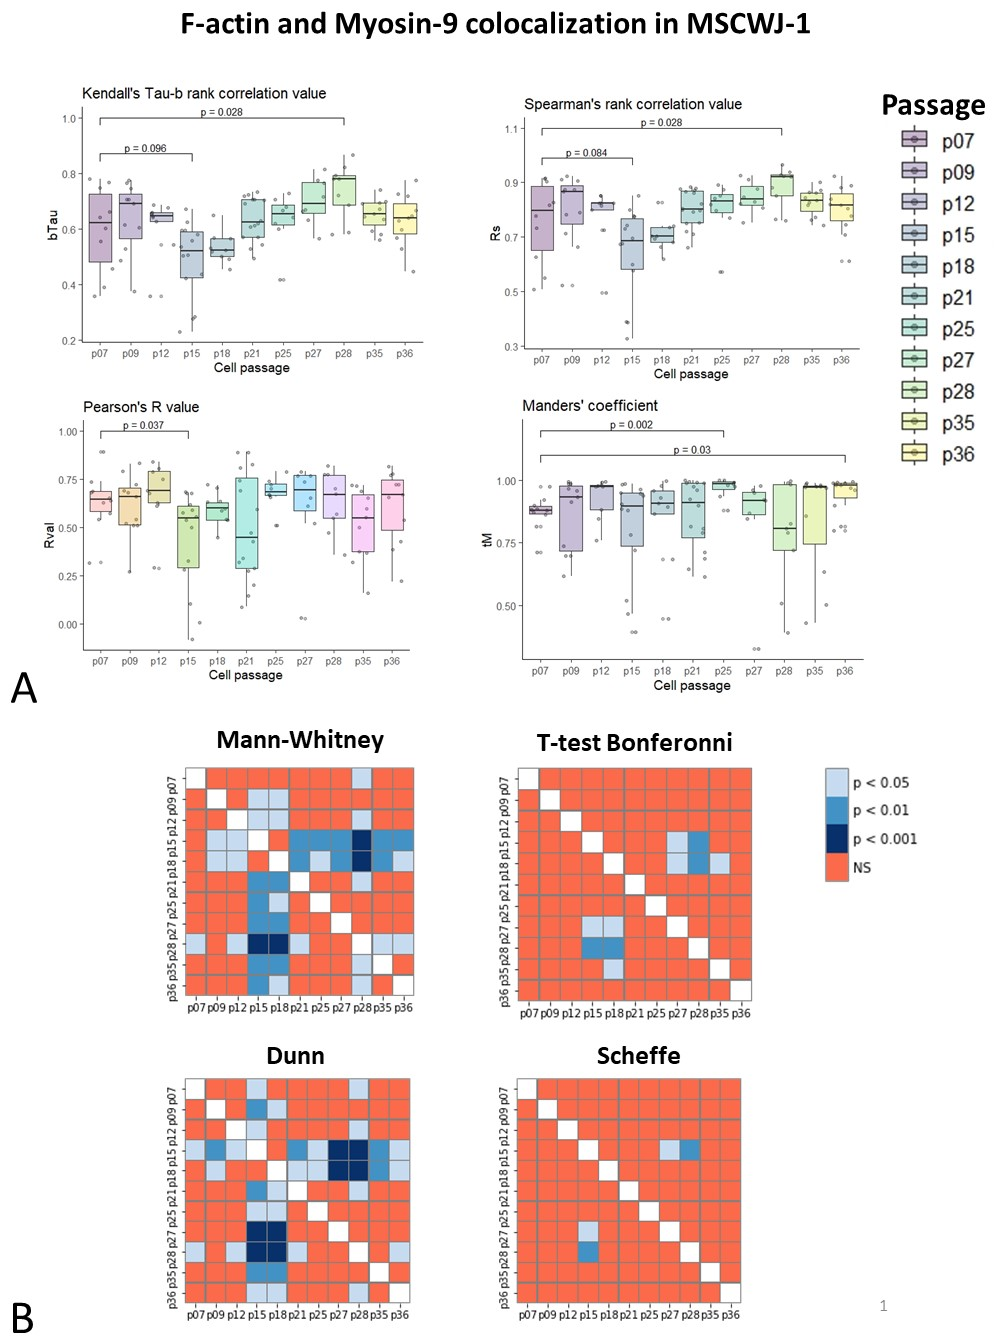
\includegraphics[width=0.9\linewidth]{fig_m9-actin-col.jpg}
\caption{F-actin and Myosin-9 Colocalization in MSCWJ-1}
\label{m9-actin-col}
\end{figure}


Kendall Miozin-9 and F-actin colocalization coefficient in р7-28р. Mean and standard error, Dynamics with confidence intervals, significant difference between groups. Pairwise t-test and t-test with Bonferroni correction.


It turns out, that Keandall and Spearman coefficients shows perfect correlation, Manders and Pearson coefficient moderate correlation (Corr = 0.758) (see supplement\ref{supp1}) ... with correlation coefficient 0.985,


\begin{figure}[hbt!]
\centering
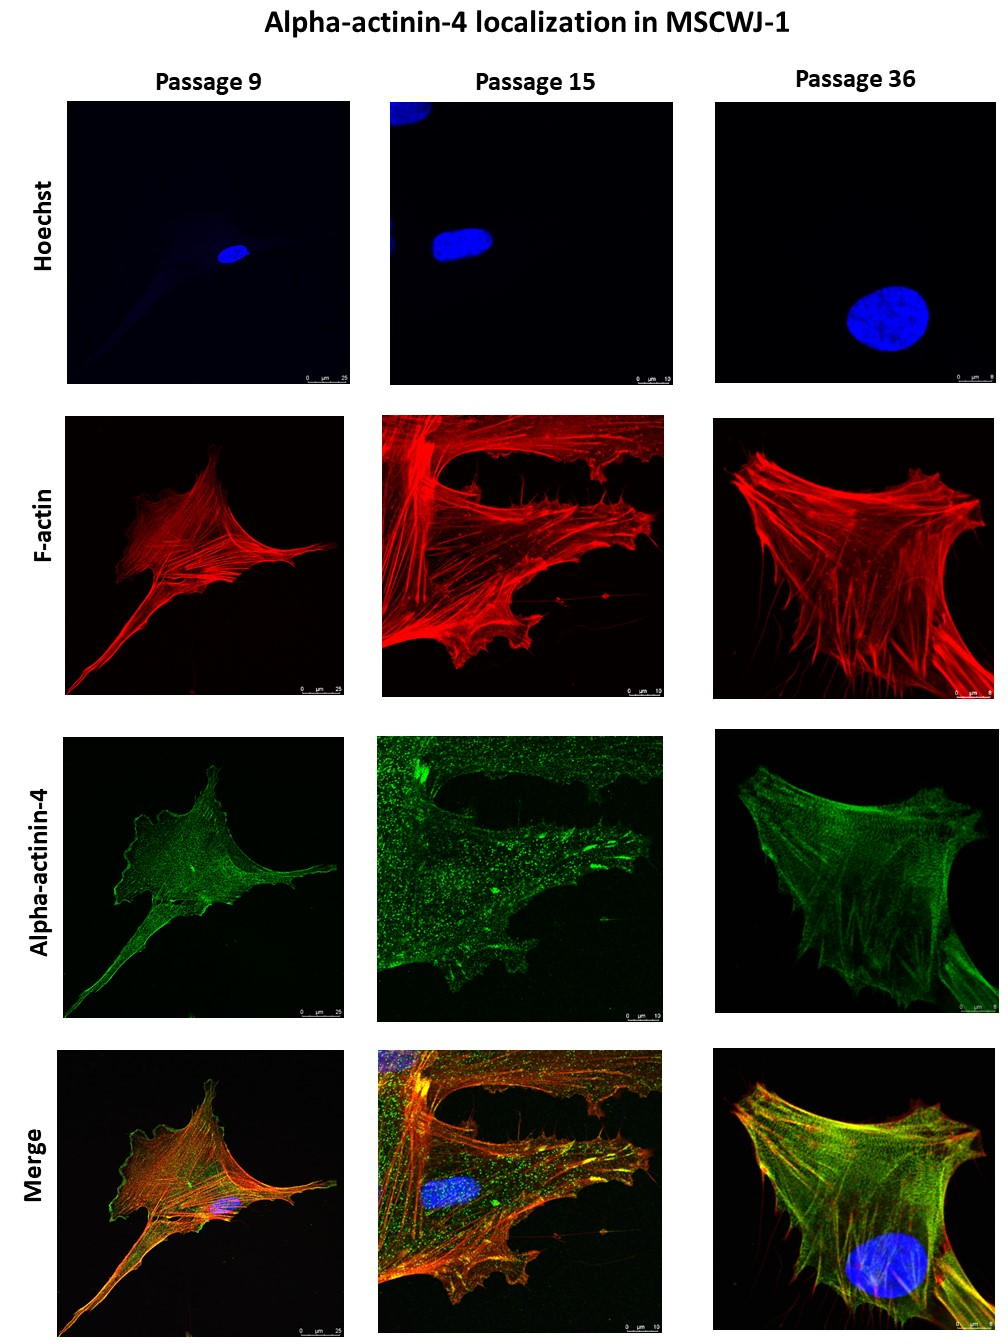
\includegraphics[width=0.9\linewidth]{fig_a4-actin.jpg}
\caption{Different passages staining of F-actin (red) and alpha-actintin-4 (green)}
\label{a4-actin}
\end{figure}



\begin{figure}[hbt!]
\centering
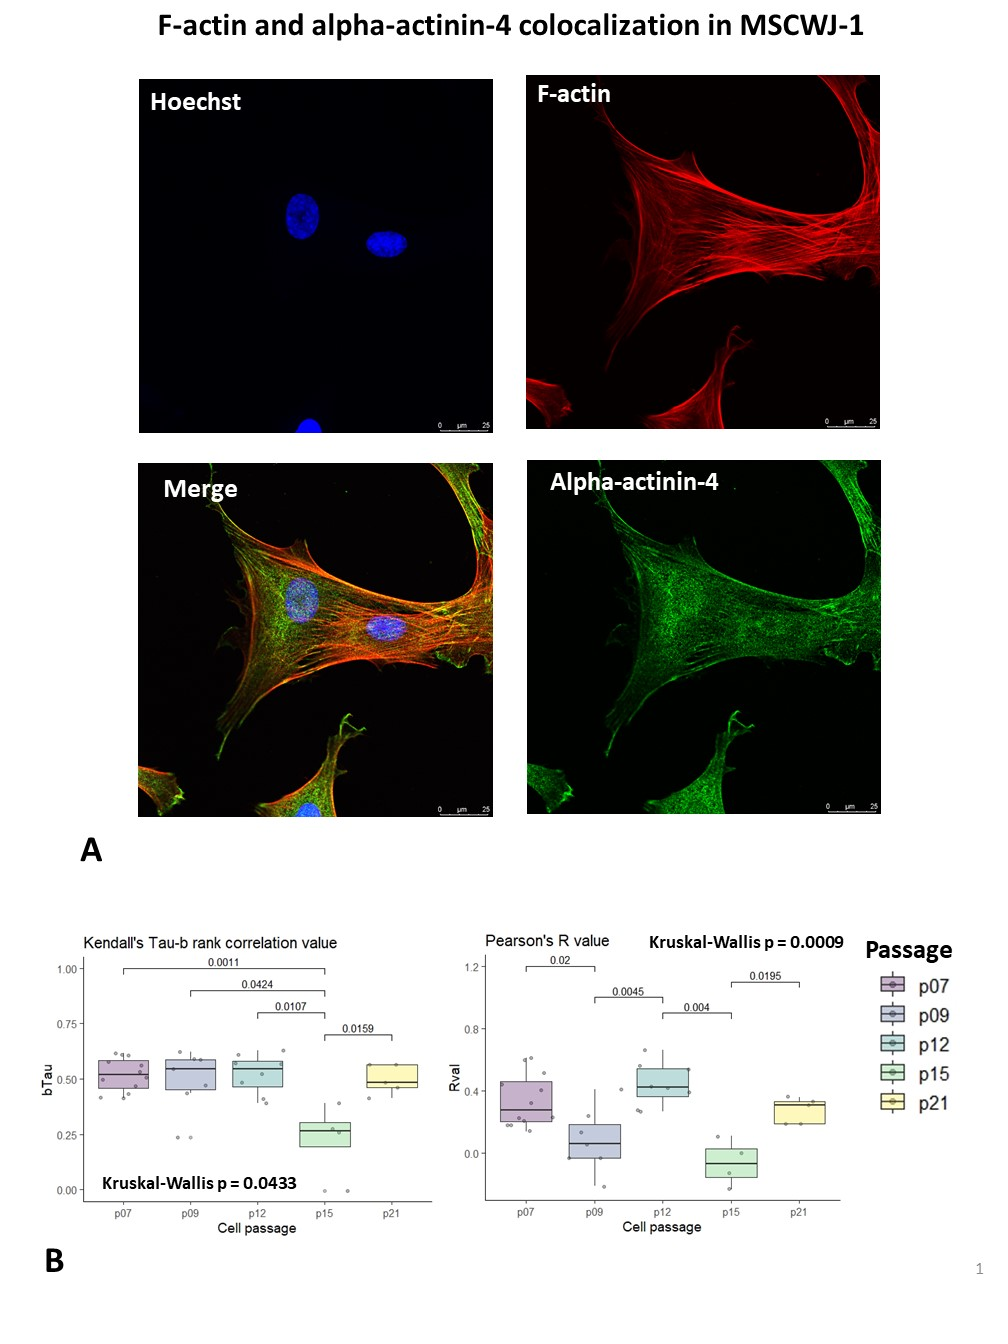
\includegraphics[width=0.9\linewidth]{fig_a4-actin-col.jpg}
\caption{Colocalization of F-actin and alpha-actintin-4 at different passages}
\label{a4-actin-col}
\end{figure}


\subsection{Colocalization of proteins}

The results of the Shapiro-Wilk test for measurements are presented in the table.
The results of the Shapiro-Wilk test indicate that the distribution of the values of the tau-Kendall rank correlation coefficient is not statistically significantly different from the normal (p> 0.05) in all groups of measurements. A multiple comparison of the medians of all samples was performed using the Kruskal-Wallis test, his results (chi-squared = 30.751, df = 8, p-value = 0.0001556) allowed to reject the null hypothesis and to conclude that there is a significant difference between the samples.
During the post hoc analysis, we used parametric Student’s two-sample t-test for independent samples to check the differences between paired samples of independent measurements by the level of the tau-Kendall rank correlation coefficient.

However, in the Shapiro-Wilk test, the p-value for the p25 sample turned out to be 0.05657, which is only slightly higher than the significance criterion chosen by us. At the same time, quantile plots show deviations from normality for high and low index values (Fig.).

Therefore, to eliminate doubts about the normality of the data, we also used the non-parametric Wilcoxon sign rank test to check the differences between paired samples of independent measurements by the level of the tau-Kendall rank correlation coefficient.


\begin{figure}
  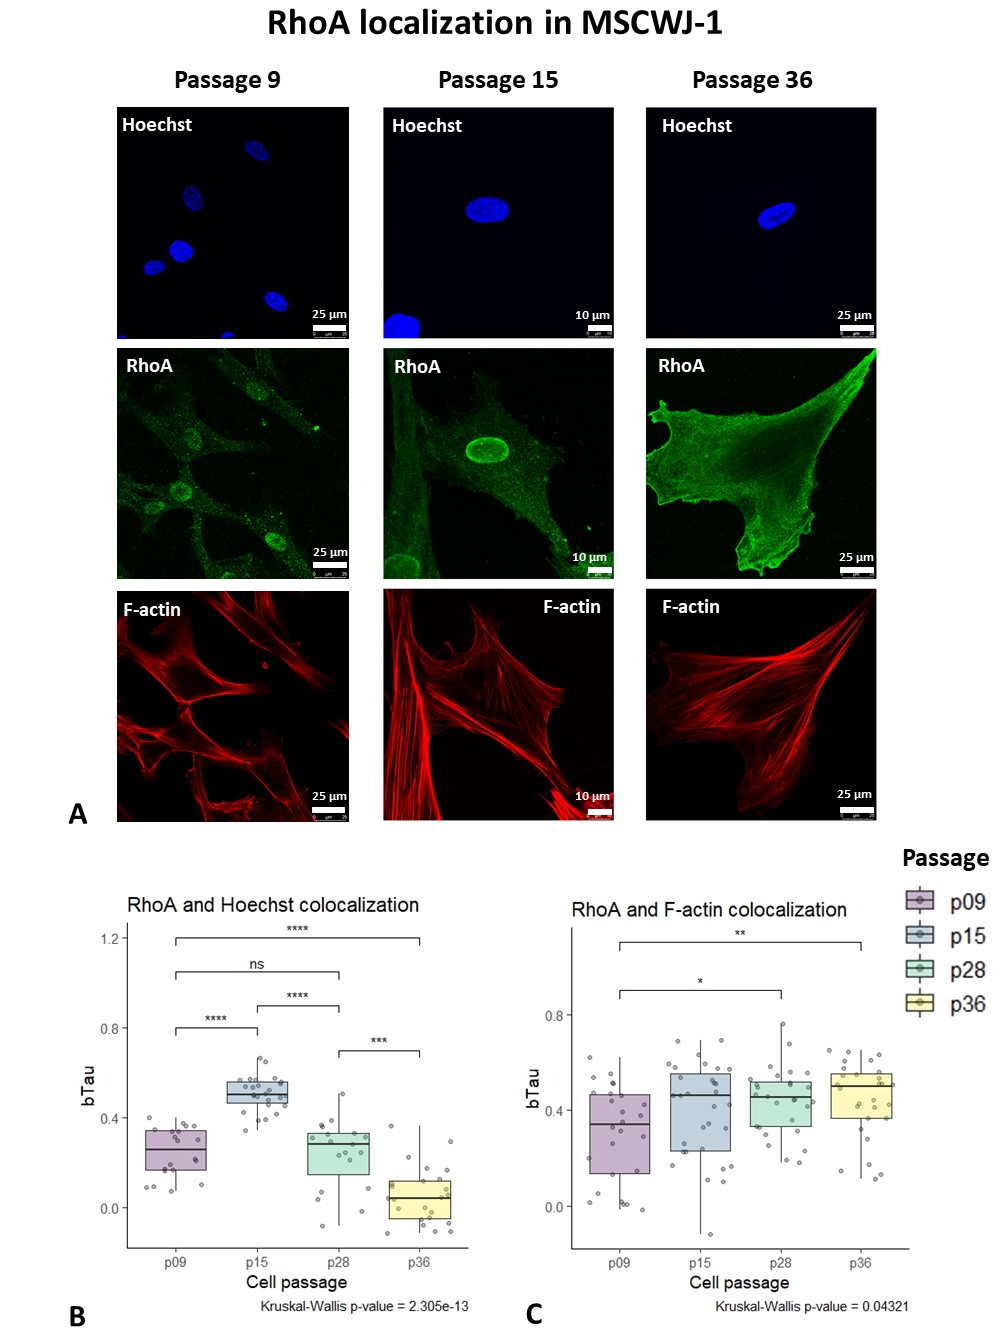
\includegraphics[width=0.9\linewidth]{fig_rho-actin-col.jpg}
  \caption{RhoA in the nucleus, along the stress In the perinuclear region, diffusely in the cytoplasm}
  \label{rho-actin-col}
  \centering
\end{figure}



\begin{figure}
  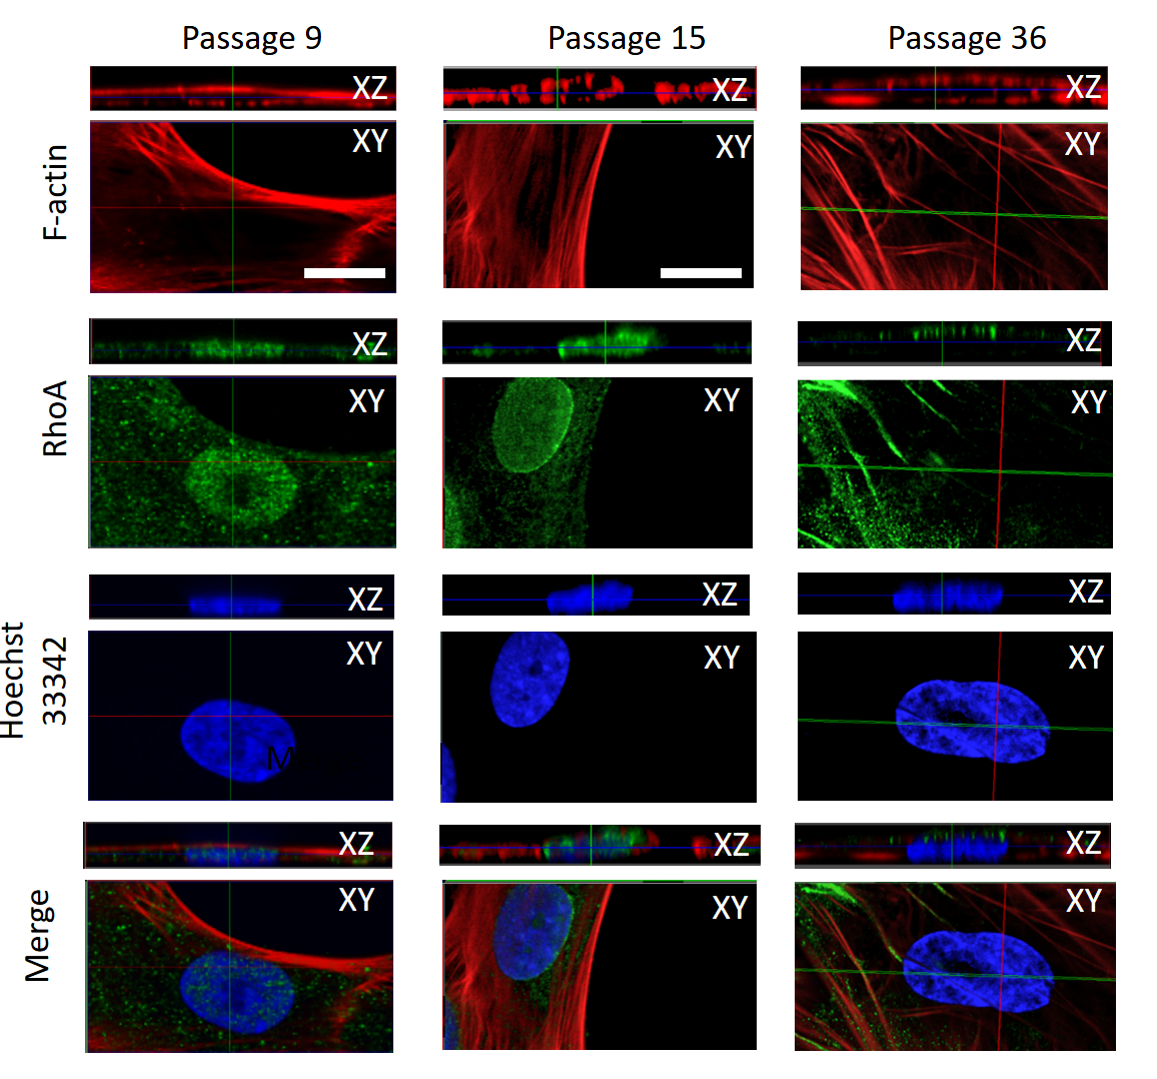
\includegraphics[width=0.9\linewidth]{fig_rho-3d.png}
  \caption{Confocal view of RhoA in the nucleus}
  \label{rho-3d}
  \centering
\end{figure}


Figure \ref{rho-3d} shows aRhoA in the nucleus...


\subsection{Trajectory analysis}


\begin{figure}
  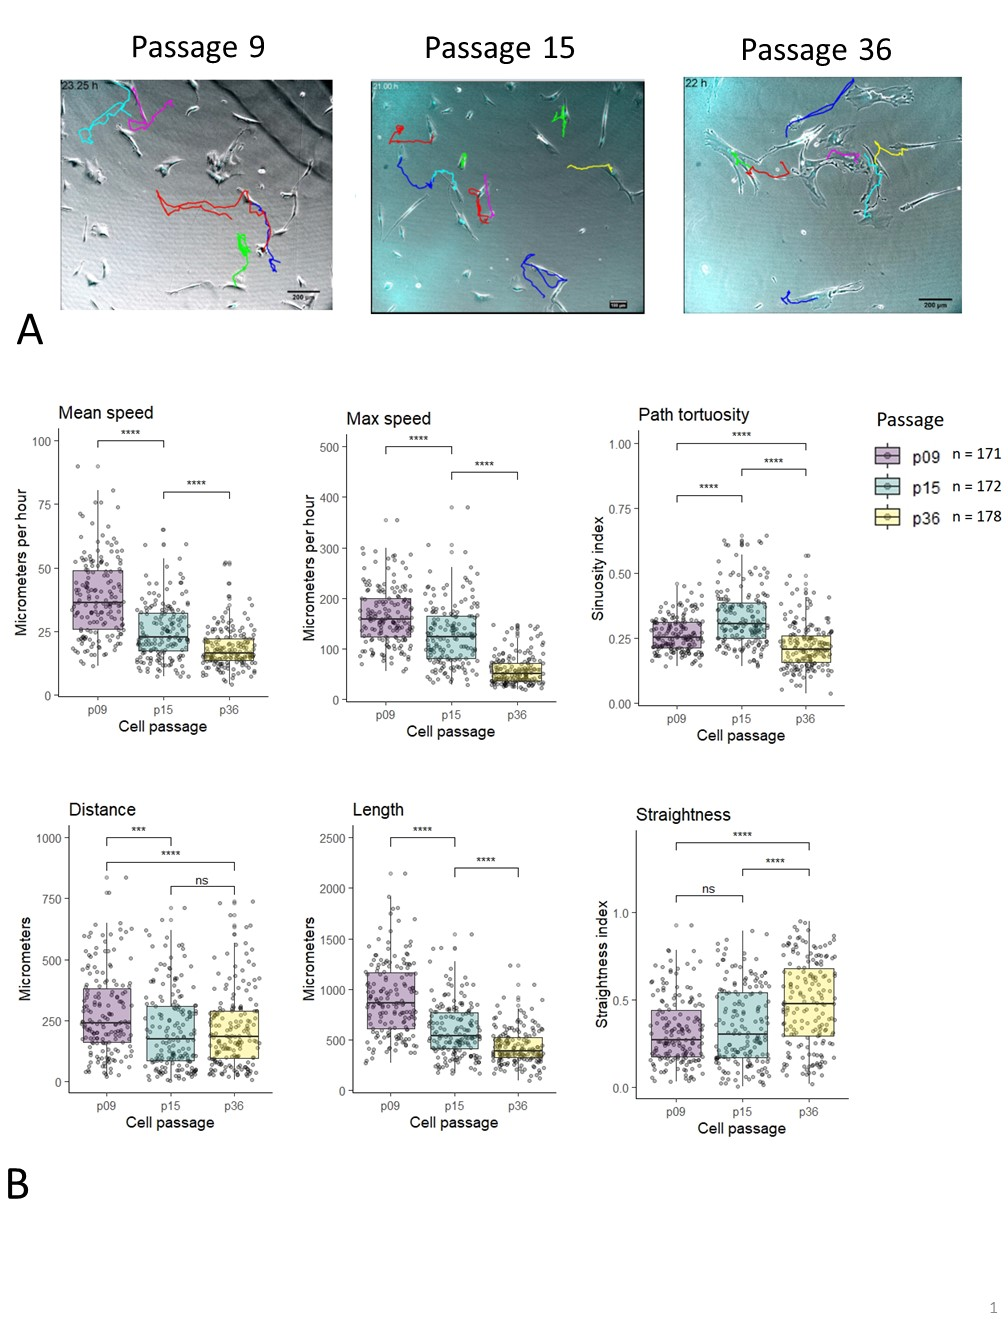
\includegraphics[width=1\linewidth]{fig_traj.jpg}
  \caption{Cell movement analisys}
  \label{traj}
  \centering
\end{figure}



\begin{table}[hb]
  \caption{24 h Trajectory analysis parameters}
  \label{tab3}
\centering
\begin{tabular}{|c|c|c|c|c|}
 \hline
 \thead{Passage} & \thead{Mean Speed, \\ $\mu$m/h} & \thead{Max Speed, \\ $\mu$m/h} & \thead{Length, \\ $\mu$m} & \thead{Distance, \\ $\mu$m} \\
 \hline
 9 & 38.3 $\pm$ 15.2 & 164.9 $\pm$ 56.4 & 911.3 $\pm$ 362.4 &  278.2 $\pm$ 169.8 \\
 15 & 25.0 $\pm$ 11.1 & 127.9 $\pm$ 59.3& 595.1 $\pm$ 263.4 & 211.7 $\pm$ 162.8  \\
 36 & 18.3 $\pm$ 7.7 & 57.1 $\pm$ 27.8 & 431.6 $\pm$ 174.5 & 215.1 $\pm$ 156.4 \\
 \hline
\end{tabular}
\end{table}

\subsection{Gel chromatography}

\begin{figure}[hbt!]
\centering
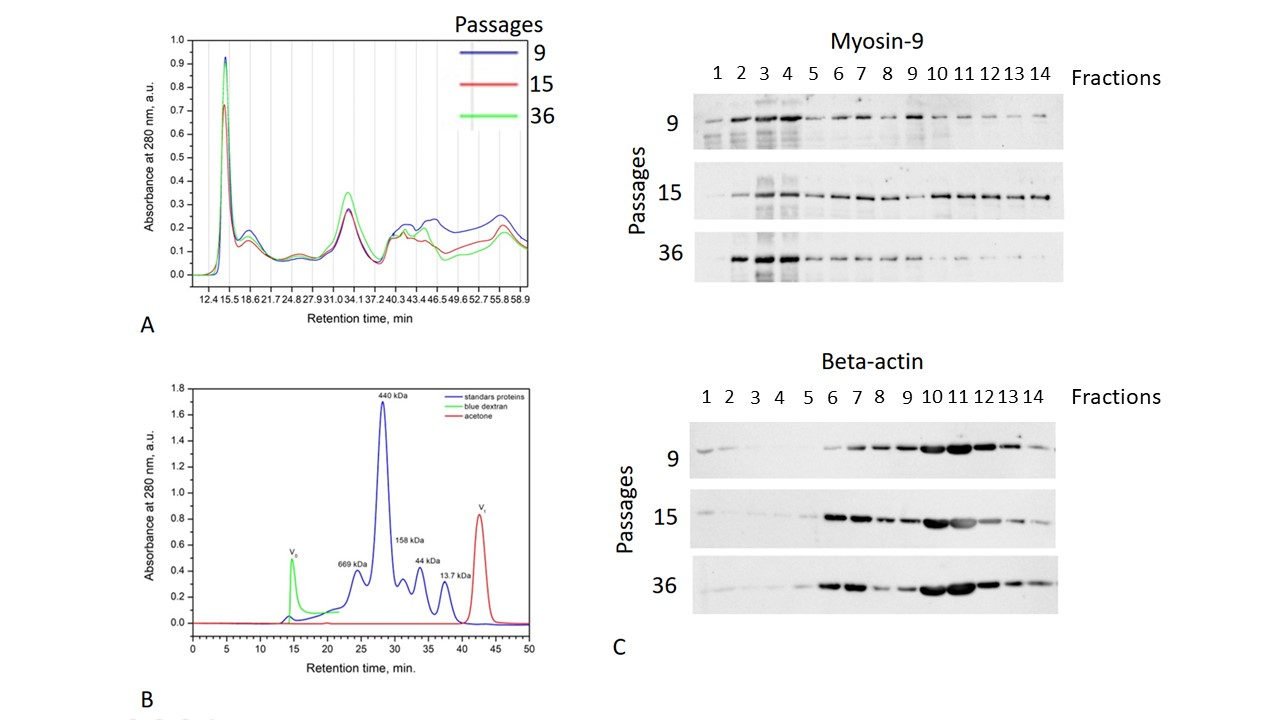
\includegraphics[width=0.9\linewidth]{fig_fplc.jpg}
\caption{Gel chromatographic separation of cytoplasmic extracts from WJ1 cells at different stages of replicative aging. Separation of calibration proteins (A) and comparison of elution profiles are presented. Fig.5 Electrophoretic separation of proteins from fractions obtained as a result of gel-chromatographic separation of cytoplasmic extracts from WJ1 cells in various stages of replicative aging.}
\label{fpcl}
\end{figure}


\section{DISCUSSION}

The actin cytoskeleton and its associated motor proteins provide the driving forces for creating amazing morphological diversity and the dynamics of mammalian cells.
Beta-galactosidase activity is expected to increase as the culture is passaged.
See table \ref{tab} for details.
From the results of Table 1, it follows that in the MSCWJ-1 line, the process of replicative aging begins with the.
Such as maintaining cell shape, its migration, interaction with the substrate and with other cells, cytogenesis, processes of intracellular transport, as well as participation in the conduct of the cellular signal and the regulation of gene expression.
Cellular actin cytoskeleton appears.
The globular actin assembly mechanism (G-actin) into threads consisting of double helix (F-actin).
Assembling and disassembling F-actin is a very dynamic process to perform various functions of actin. Similar dynamics are regulated by a number of actin-binding and regulatory proteins.
Thus, there are mechanisms that prevent the spontaneous polymerization of G-actin into filaments by the relative instability of actin dimer or trimer and G-actin-binding and sequestering proteins, such as profilin and $\beta$-thymosin, respectively (....).
On the other hand, a number of actin-binding proteins prevent the depolymerization of F-actin microfilaments and regulate their stability (such as tropomyosin, alpha-actinin, for example).
A recent study has shown that targeting and activation of actin filament nucleators (gelsolin), elongators, and myosin engines are closely coordinated by conservative protein complexes to orchestrate the generation of power. (\cite{pantaloni1993profilin}; \cite{sept2001thermodynamics}).
The distribution of these and many other structures in the cell allows you to perform all the variety of the above listed functions.
To establish the many different actin assembly functions required in time and space, actin nucleators target specific subcellular compartments, thereby limiting the formation of specific structures of actin filaments to these sites.
Cellular aging, replicative cycle, Hayflick limit.
Currently, two main theories about the mechanisms of aging are competing with each other: telomeric and oxidative (it is free radical, it is mitochondrial). In 1961, an American doctor, Leonard Hayflick, discovered that human cells cannot endlessly divide: in vitro they undergo approximately 50 doublings and stop proliferation (\cite{hayflick1961serial}).
This figure of 50 doublings, called the Hayflick limit, is fairly arbitrary, since it is not possible to accurately determine how many times a single human cell can share.
Thus, the results of Hayflick's experiments do not mean that the human cell is able to share exactly 50 times (most likely more), but only mean that with the counting method that Hayflik used and which is used now as the simplest and most convenient, a population of human fibroblasts in culture doubles usually ~ 50 $\pm$ 10 times.
Cell cycle arrest during replicative aging.


Another structure characteristic mainly of non-muscle cells is stress fibrils — bundles of F-actin filaments stabilized by such proteins.
Features of the organization of the actin cytoskeleton in mesenchymal stem cells.
The most important population of adult stem cells are mesenchymal stem cells (MSCs).
For the first time, these cells were detected and isolated from the bone marrow stroma.
It was believed that bone marrow MSCs serve as a source for the renewal and restoration of connective tissues such as bone, cartilage and adipose.
At present, analogs of bone marrow MSC are found in all other tissues.
Thanks to the approaches that allow identifying MSCs in situ, isolating them from tissues and finally evaluating biological properties, it became possible to revise the role of MSCs in various organs and tissues.
This review summarizes our own and published data on the role of MSCs in the processes of repair and tissue regeneration.
In our opinion, MSCs perform the function of conjugating the circulatory, immune, hormonal, and nervous systems with tissue-specific stem cells.


Elliott et al. find that Rho/ROCK-stimulated myosin II contractility minimizes cell-scale branching by recognizing and minimizing local cell-surface curvature \cite{elliott2015myosin}.
Differences in the organization of the cytoskeleton in normal and cancer cells (\cite{shutova2010normal}).
The cell movement is based on the rearrangement of the actin cytoskeleton. The initial step of the rearrangements is the formation of the so-called leading (active) edge, at which protrusions take place and primary contacts of the cell with the extracellular matrix are formed. Protrusion of the leading edge is provided by the force of polymerization of actin in the zone of the lamellipodia. In the lamella zone, a further rearrangement of actin takes place - the formation of actin-myosin beams. The formation of contacts with the substrate is initiated in the lamellipodia, and maturation occurs in the lamella zone with the participation of stress-fibrils (Alexandrova et al., 2008).
The tension generated by myosin affects the initial focal complexes, inducing their growth and transformation into focal contacts (Ingber, 1991; Riveline et al., 2001; Rottner et al., 2001; Krendel, Mooseker, 2005) .
A striking example of the dynamic organization of the cytocell is its restructuring, occurring in the cell spreading process. The process of spreading begins with the formation of pseudopodia around the entire perimeter of the cell.
The network of microfilaments on the active edge is constantly formed during the entire spreading process due to the intense polymerization of actin.
The remaining types of actin-containing structures arising in sprawling cells are mainly the result of a sequential reorganization of actin polymerized at the edges. The first stage of such a rearrangement is the emergence of an annular beam located along the edge of the discoid cell immediately behind the zone of the active edge (radial spreading stage) (Svitkina et al., 1986).
In the case of fibroblast-like cells, the spreading process on the substrate ends with the stage of polarization. Fibroblasts acquire an elongated polarized form as a result of the redistribution of pseudopodial activity - the division of the cell edge into active and stable zones (Rivne, Vasiliev, 2004).
Neoplastic transformation disrupts normal morphogenetic reactions and cell mobility, leading to processes such as invasive growth and metastasis (Rovno, Vasiliev, 2004).
Reorganization of the cytoskeleton, especially changes in cell contractility, regulated by the actin-myosin complex, is of central importance for the development of the phenotype of morphologically transformed cells with invasive behavior.
The reduction of stress-fibrils, characteristic of many types of transformed cells, is associated with impaired maturation of contact structures (Rovno, Vasilyev, 2004) and often correlates with an increase in locomotor activity and / or metastatic potential of tumor cells (Pokorna et al ., 1994; Sahai, Marshall, 2002).
The transformed cells in the culture are observed violations of spreading.
At all stages of spreading, the distribution of lamellipodia is disturbed, as a result of which lamellae are formed as separate fragments, and not along the entire perimeter of the cell. Flattening of the cell is uneven, disc-shaped is not observed.
Upon completion of the spreading, such cells do not reach a large area comparable to the area of normal cells (Rovensky, Vasiliev, 2004).
In order to give a structural interpretation to the immunofluorescence data we investigated changes in distribution of cytosole-derived myosin-9 in FPLC gel-filtration fractions.
Apparently, the accumulation of myosin-9 in light molecular weight fractions after gel filtration, which we observe at passage 15, is due to the fact that the protein is in the assembly-incompetent form (\cite{vicente2009non}), which is also consistent with immunofluorescence data, where we see the accumulation of actin-binding proteins in the form of individual particles, or multimolecular protein complexes.
\cite{shutova2018mammalian}
These data can be compared with the results of the analysis of cell motility, in which the sinuosity index reaches its maximum at passage 15, which indicates that such cells change direction of movement more often than young and old cells.

Apparently, the contribution of cells with a predominant amoeboid type of movement becomes so noticeable.
It is possible that switching from the mesenchymal type of movement and vice versa is mediated by the transfer of myosin-9 from one form to another and requires the presence of RhoA in the nucleus.
Moving to the nucleus,RhoA can down-regulate stress fibrils organization and at the same time regulate a number of genes.


\section*{Conclusion}

Sed ut perspiciatis unde omnis iste natus error sit voluptatem accusantium doloremque laudantium, totam rem aperiam, eaque ipsa quae ab illo inventore veritatis et quasi architecto beatae vitae dicta sunt explicabo.

Replicative aging of human mesenchymal stem cells is accompanied by changes in the organization of the contractile apparatus.

\section*{Author Contributions}

Author2 designed the research. Author1 carried out all simulations, analyzed the data. Author1 and Author2 wrote the article.

\section*{Acknowledgments}

We thank G. Harrison, B. Harper, and J. Doe for their help.

%\bibliographystyle{plain}
%\bibliographystyle{plainnat}
%\bibliographystyle{apacite}
\bibliographystyle{apalike}
\bibliography{mybib}
\section*{Supplementary Material}

\subsection{Superose 6 column calibration kit}

\begin{table}[h]
  \caption{Gel-filtration calibration protein set}
  \label{calibration}
\centering
\begin{tabular}{l|c|}
 Protein & Molecular weight (Mr), kDa  \\
 \hline
 Ovalbumin & 43 \\
 Horse spleen Thyroglobulin & 669 \\
 Rabbit muscle Ferritin & 440 \\
 Chicken egg white Aldolase & 158 \\
 Bovine erythrocytes Ovalbumin & 43 \\
 Bovine lung Ribonuclease A & 13.7
\end{tabular}
\end{table}

\subsection*{Video files}

Video files with cell tracking...

\subsection*{Tables in csv format}

alltracks.csv

\subsection*{Colocalization coefficients correlation analisys}

The supplement presents the dependence of the studied parameters from each other, in the form of a matrix.
Vertically and horizontally, the correlation coefficients are plotted that we calculated for myosin-9 and actin, there are 5 in total: Rs, Rval, tM1, tM2, bTau (these are the Spearman, Pearson, Manders, and Kendall correlation coefficients).
And the work presents the results for bTau and Rval.
Different coefficients give a slightly different picture of the distribution of means in the measurements, well, this table in the appendix justifies our choice of these bTau and Rval.
In particular, it can be seen that, for example, Rs and bTau are almost the same thing, and in order to get rid of redundancy, we can only talk about one of them, so we choose bTau.
In the article in fig. 2B, a small plate remains with correlation values ​​between the measured solocalization coefficients.

\begin{figure}[h]
  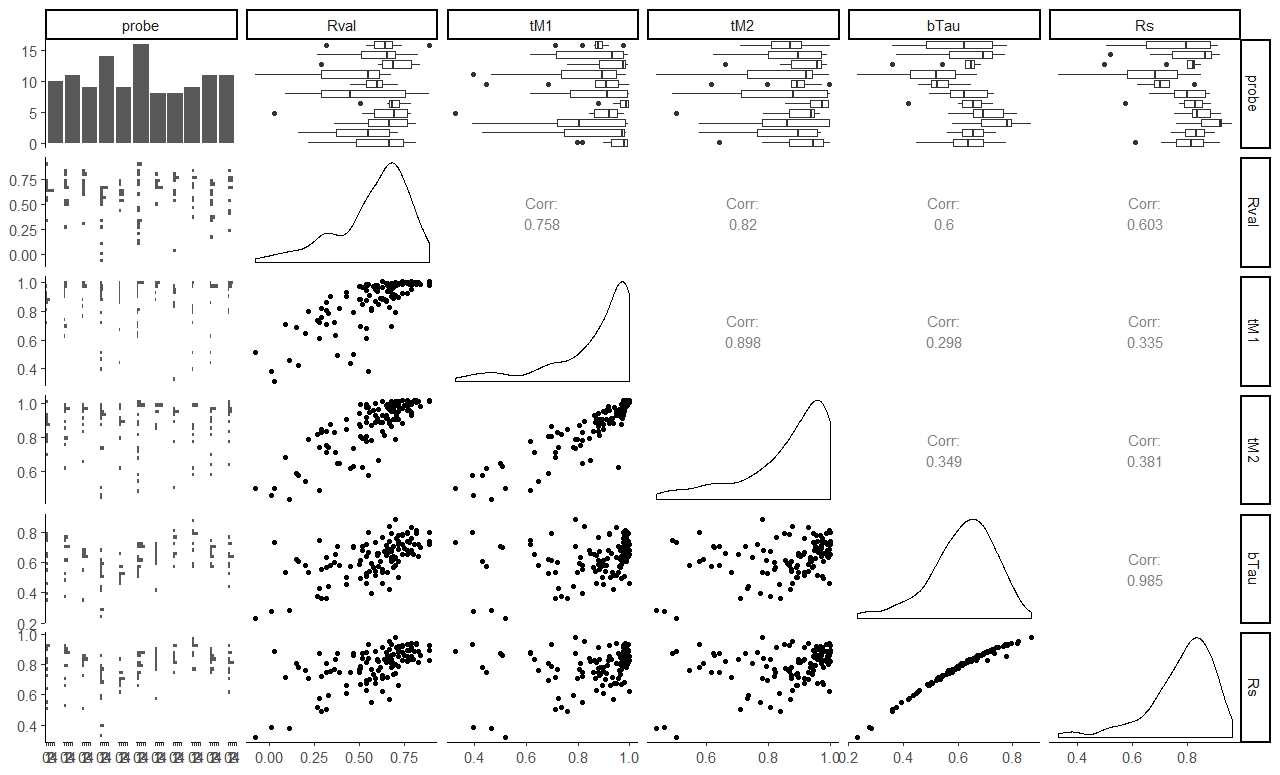
\includegraphics[width=1\linewidth]{supp1.jpeg}
  \caption{Matrix of plots with a data set containing myosin-9/F-actin colocalization coefficients.}
  \label{supp1}
  \centering
\end{figure}

\begin{table} [h]
  \caption{Kruskal-Wallis rank sum test results for myosin-9 and F-actin colocalization coefficients}
  \label{tab1}
\centering
\begin{tabular}{l|ccc}
 Colocalization coefficient & chi-squared & df & p-value  \\
 Kendall's Tau-b & 34.669 & 10 & 0.0001422 \\
 Spearman's R & 34.373 & 10 &  0.0001596 \\
 Manders' M & 16.107 & 10 & 0.09661 \\
 Pearson's R & 15.152 & 10 & 0.1266

\end{tabular}
\end{table}

% latex table generated in R 3.6.1 by xtable 1.8-4 package
% Sat Aug 17 01:43:09 2019

\begin{table}[ht]
  \caption{Fitting Generalized Linear Models family = "binomial"}
  \label{glm}
\centering
\begin{tabular}{lrrrrr}
  \hline
 & Df & Deviance & Resid. Df & Resid. Dev & Pr($>$Chi) \\
  \hline
NULL &  &  & 115 & 68.13 &  \\
  Rval & 1 & 0.95 & 114 & 67.18 & 0.3295 \\
  tM1 & 1 & 0.91 & 113 & 66.27 & 0.3407 \\
  tM2 & 1 & 1.32 & 112 & 64.96 & 0.2510 \\
  bTau & 1 & 4.14 & 111 & 60.82 & 0.0419 * \\
  Rs & 1 & 0.20 & 110 & 60.61 & 0.6509 \\
   \hline
\end{tabular}
\end{table}

% latex table generated in R 3.6.1 by xtable 1.8-4 package
% Mon Aug 19 18:16:31 2019
\begin{table}[hb]
  \caption{Logistic regression with colocalization coefficients as predictors and passage numger as fitted values}
  \label{glm-RhoA-nuc}
\centering
\begin{tabular}{l|rrrr}
  \hline
 & Estimate & Std. Error & z value & Pr($>$$|$z$|$) \\
  \hline
(Intercept) (**) & 2.2687 & 0.7100 & 3.20 & 0.0014 \\
  bTau (***) & 97.1021 & 27.8353 & 3.49 & 0.0005 \\
  Rval & 0.5242 & 1.3355 & 0.39 & 0.6947 \\
  Rs (***) & -78.1599 & 22.1536 & -3.53 & 0.0004 \\
   \hline
\end{tabular}
\end{table}


\end{document}
